\documentclass[11pt]{beamer}
%\setbeamertemplate{frametitle}
%{\begin{centering}\smallskip
%   \insertframetitle\par
%   \smallskip\end{centering}}
%\setbeamertemplate{itemize item}{$\bullet$}
%\setbeamertemplate{navigation symbols}{}
%\setbeamertemplate{footline}[text line]{%
%\hfill\strut{%
%        \scriptsize\sf\color{black!60}%
%        \quad\insertframenumber
%     }%
%\hfill
%}

\usepackage[utf8]{inputenc}
\usepackage{amsmath}
\usepackage{amsfonts}
\usepackage{amssymb}

\usepackage[brazil]{babel}
\usepackage{subfig}

% Evita Warning Font shape `OT1/cmss/m/n' in size <4> not available(Font) size <5> substituted
\usepackage{lmodern}

\usepackage{tikz}
\usepgflibrary{arrows}% for more options on arrows

\author{\mbox{Rafael Pereira Lima} \and
		\mbox{Orientador: Prof. Dr. Carlos Hitoshi Morimoto}}
\title{Rastreamento de Olhar Usando Compressive Sensing}
\subtitle{Trabalho de formatura}
%\setbeamercovered{transparent} 
%\setbeamertemplate{navigation symbols}{} 
%\logo{} 
\institute{IME-USP} 
\date{8 de dezembro de 2016} 
\subject{} 

\captionsetup{labelformat=empty,labelsep=none}%remove prefixo 'Figura' em caption

\setbeamertemplate{footline}{\hfill\insertframenumber/\inserttotalframenumber} 

\begin{document}

\begin{frame}
\titlepage
\end{frame}

\begin{frame}
\frametitle{Rastreamento de olhar}
Rastreamento de olhar consiste na determinação da posição do olhar em determinado período.
\begin{figure}
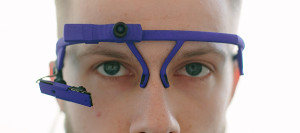
\includegraphics[scale=1]{imagens/dmk-headset.jpg}
\caption{\tiny{\url{https://pupil-labs.com/blog/2016-07/new-headset-color/}}}
\end{figure}
\end{frame}

\begin{frame}
\frametitle{Rastreamento de olhar}
\framesubtitle{Aplicações}
\begin{figure}
	%\subfloat{
\includegraphics[scale=.5]{imagens/deficientes.png} }
	\subfloat{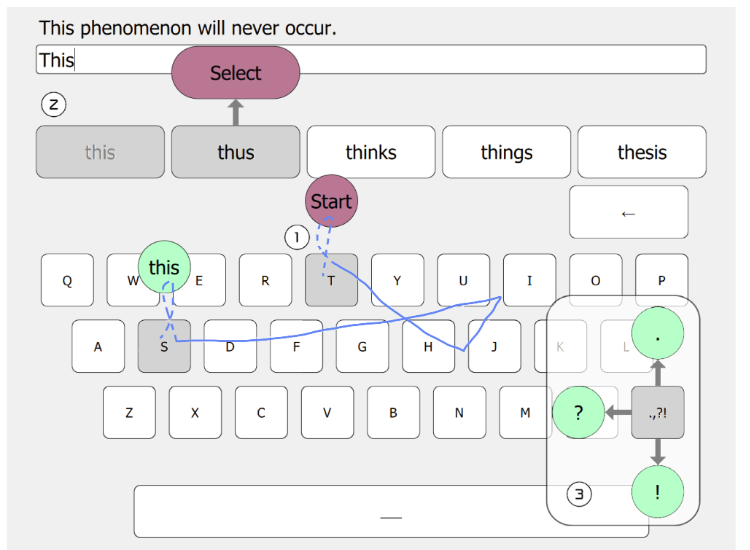
\includegraphics[scale=.3]{imagens/teclado.png}}
	\caption{\tiny{Kurauchi, Andrew, et al. "EyeSwipe: Dwell-free Text Entry Using Gaze Paths." Proceedings of the 2016 CHI Conference on Human Factors in Computing Systems. ACM, 2016.}}
\end{figure}
\end{frame}

\begin{frame}
\frametitle{Rastreamento de olhar}
\framesubtitle{Aplicações}
\begin{figure}
	\subfloat{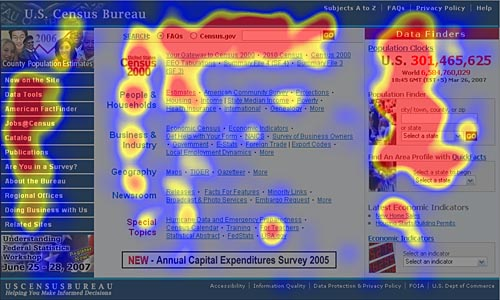
\includegraphics[scale=.4]{imagens/census-homepage-heatmap.jpg} }
	\caption{\tiny{\url{https://www.nngroup.com/articles/fancy-formatting-looks-like-an-ad/}}}
\end{figure}
\end{frame}

\begin{frame}
\frametitle{Rastreamento de olhar}
\framesubtitle{Aplicações}
\begin{figure}
	\subfloat{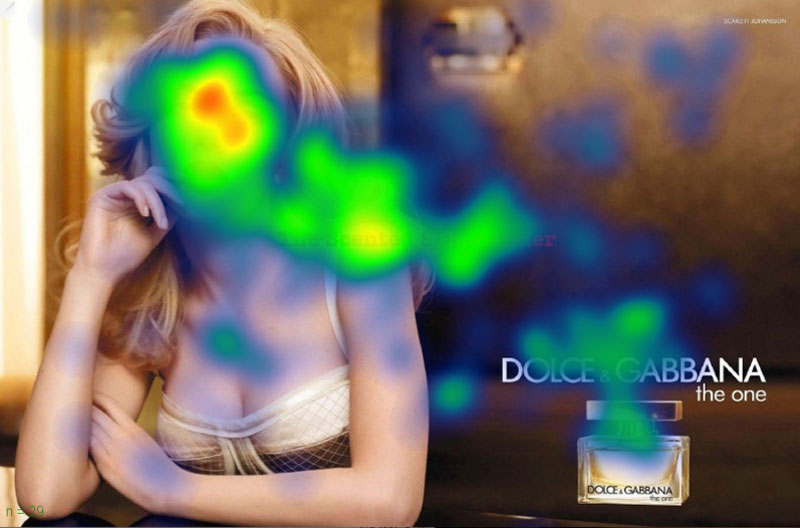
\includegraphics[scale=.3]{imagens/dolcegabbana.jpg} }
	\caption{\tiny{\url{http://www.businessinsider.com.au/eye-tracking-heatmaps-2014-7}}}
\end{figure}
\end{frame}

\begin{frame}
\frametitle{Rastreamento de olhar}
\framesubtitle{Rastreamento baseado em vídeo}
\begin{columns}[t]
\column{.5\textwidth}
\centering
\hspace{10cm}
\begin{figure}
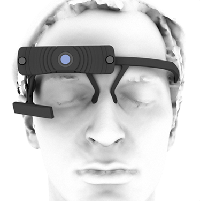
\includegraphics[scale=.6]{imagens/pupil.png}
\caption{\tiny{\url{https://pupil-labs.com/blog/2014-01/new-pupil-pro-headset-capture-software-0-3-7/}}}
\end{figure}
\column{.5\textwidth}
\centering
Imagem do olho em RGB
\begin{figure}
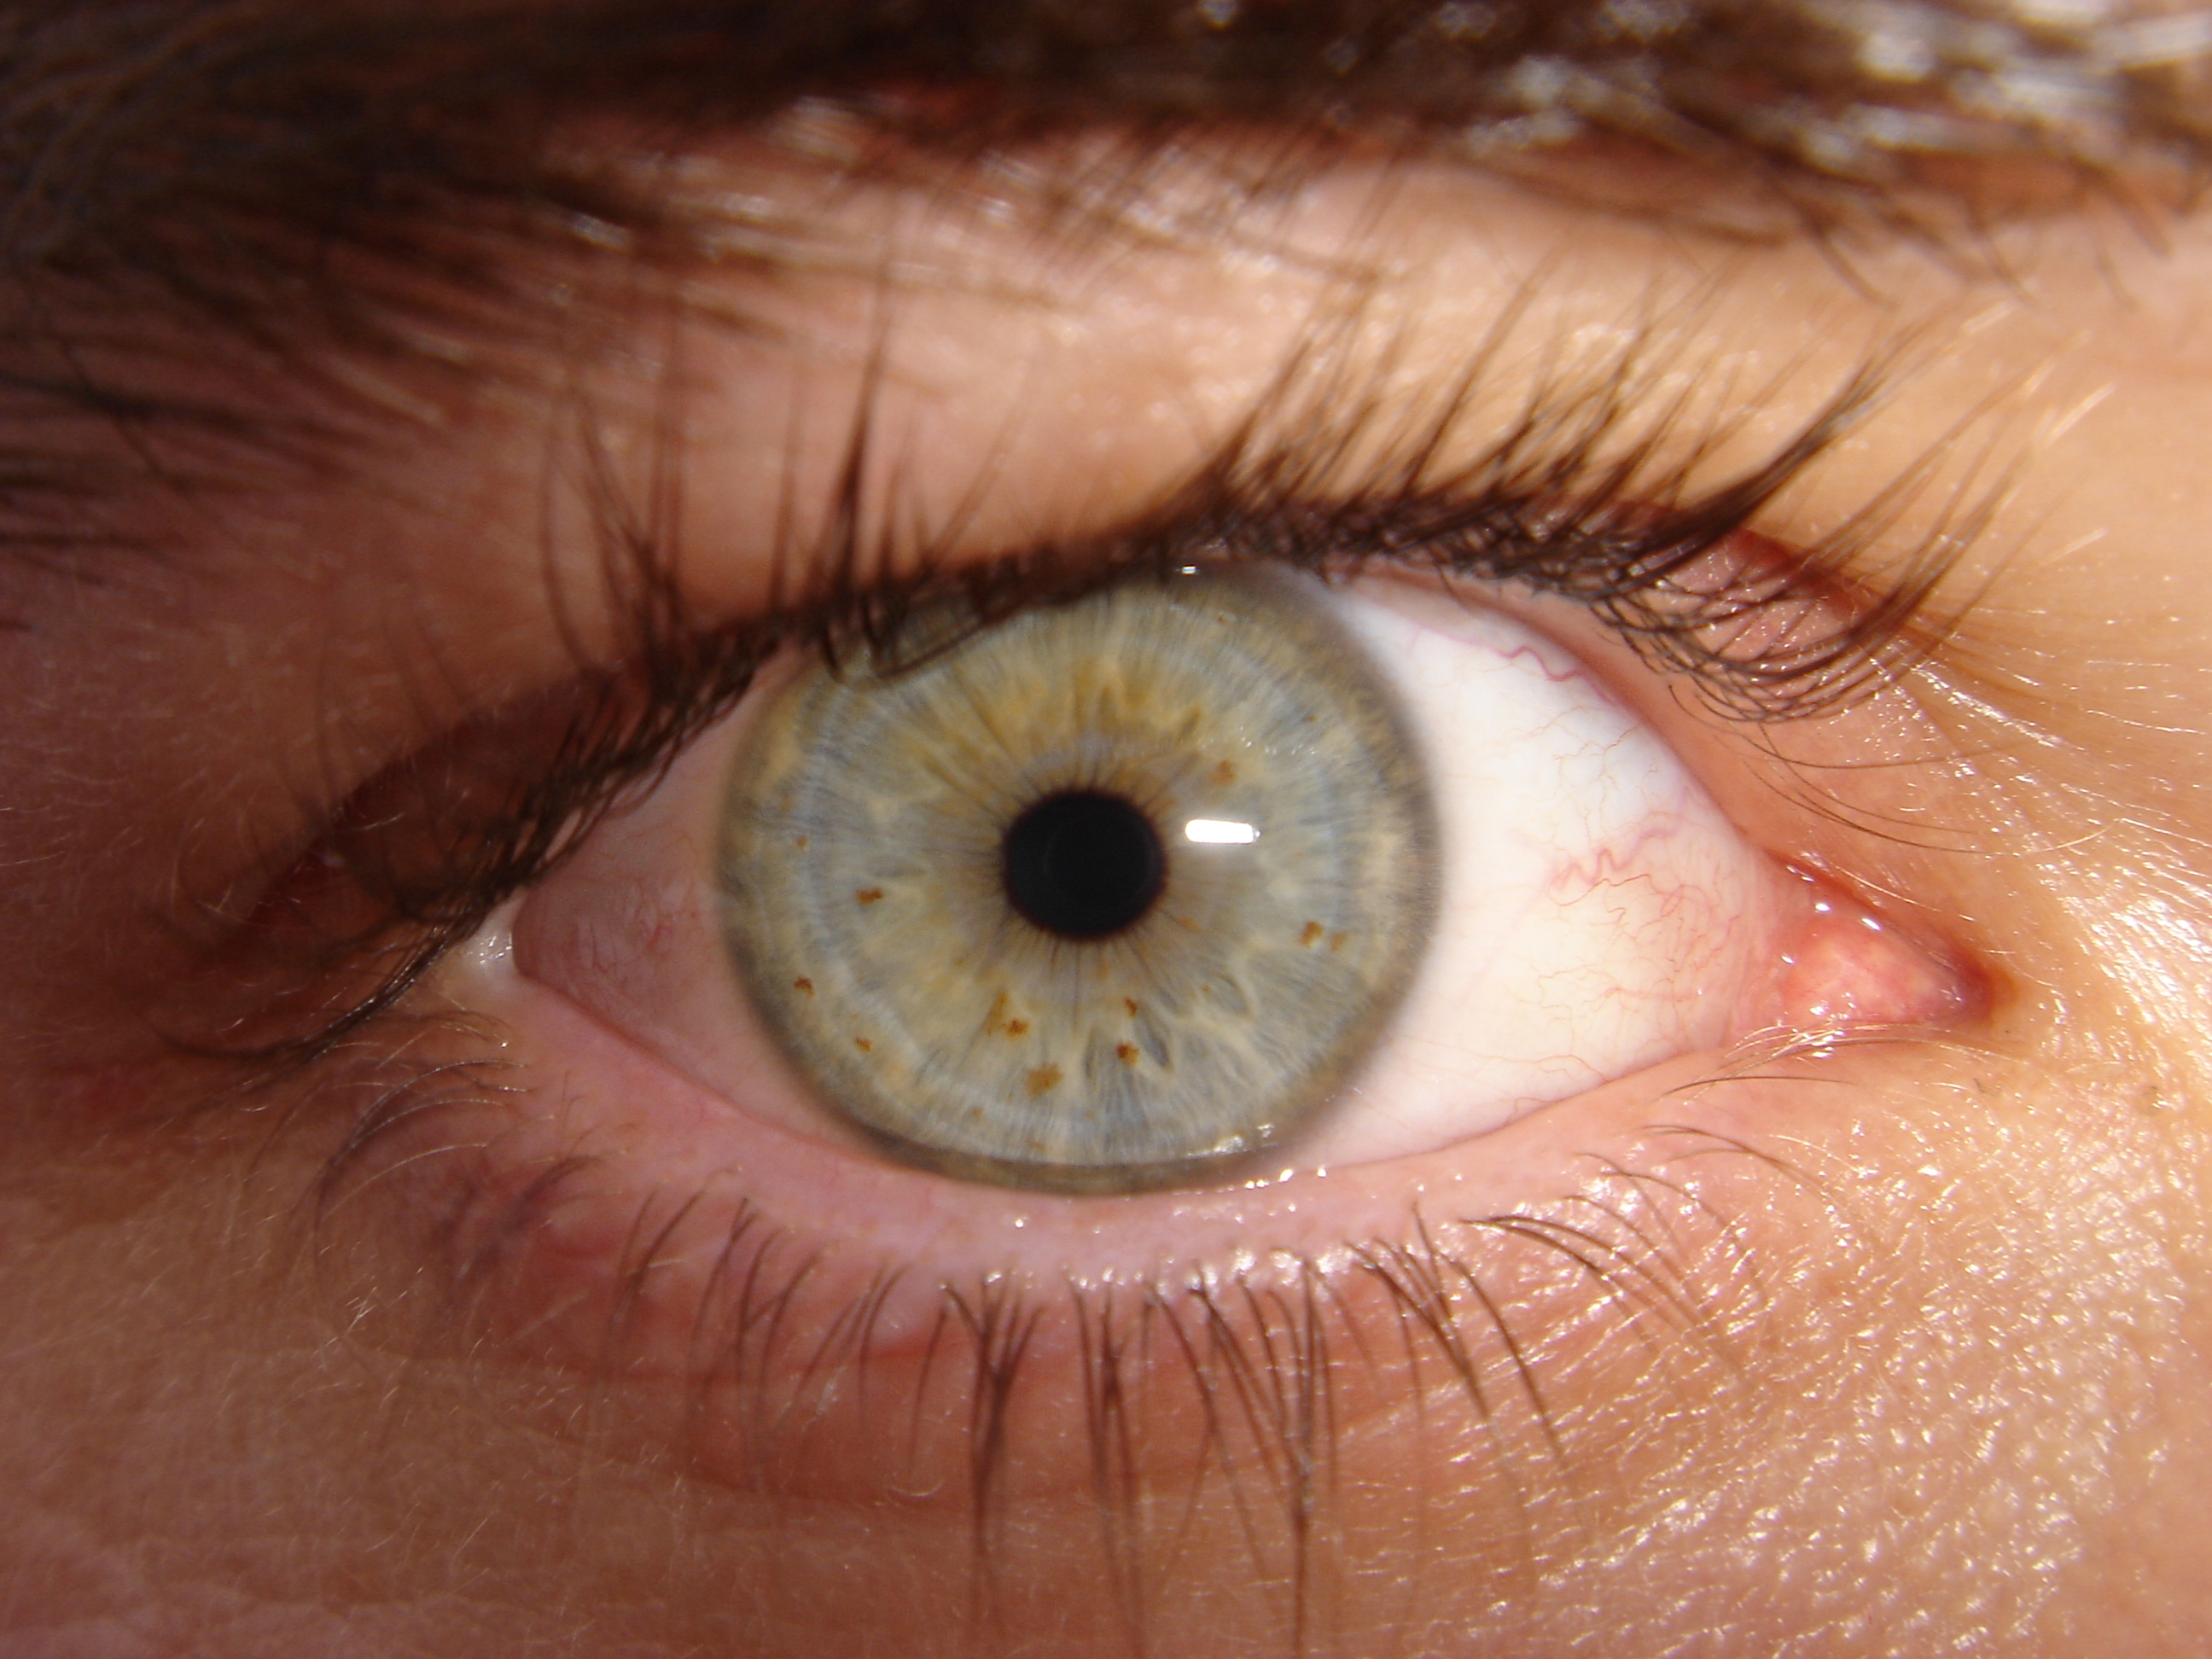
\includegraphics[scale=.03]{imagens/Myeye.jpg}
\caption{\tiny{\url{https://commons.wikimedia.org/wiki/File:My_eye.jpg}}}
\end{figure}
\vspace{.2cm}
Imagem  em Infravermelho\\
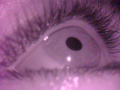
\includegraphics[scale=.65]{imagens/26.jpg}
\end{columns}
\end{frame}

\begin{frame}
\frametitle{Rastreamento de olhar}
\framesubtitle{Rastreamento baseado em vídeo}
\begin{columns}[t]
\column{.5\textwidth}
\centering
\textit{Head-mounted}
\begin{figure}
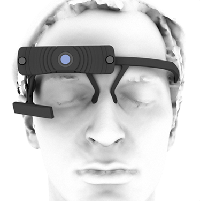
\includegraphics[scale=.6]{imagens/pupil.png}
\caption{\tiny{\url{https://pupil-labs.com/blog/2014-01/new-pupil-pro-headset-capture-software-0-3-7/}}}
\end{figure}
\column{.5\textwidth}
\centering
\textit{remoto}
\begin{figure}
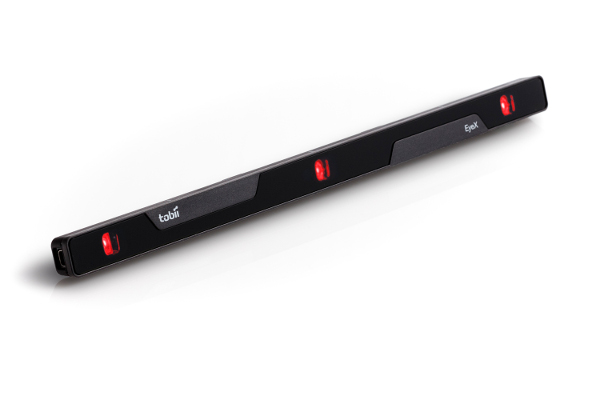
\includegraphics[scale=1]{imagens/eyex.jpg}
\caption{\tiny{\url{http://www.tobii.com/group/news-media/press-releases/2015/12/tobii-validated-for-windows-hello-}\\\url{login-announces-support-for-facial-recognition/}}}
\end{figure}
\end{columns}
\end{frame}

\begin{frame}
\frametitle{Compressive Sensing}
Compressive Sensing(CS), ou Compressed Sensing, estuda formas de reconstruir um vetor $x$ com

$$ Ax = y$$

onde $A$ é $m \times n$ e $m \ll n$.
\end{frame}

\begin{frame}
\frametitle{Compressive Sensing}
Poderíamos tentar o método dos mínimos quadrados:

$$\min_{x \in \mathbb{R}^n} \Vert Ax - y \Vert_2^2$$

mas

\begin{columns}[t]
\column{.5\textwidth}
\begin{center}
\begin{figure}
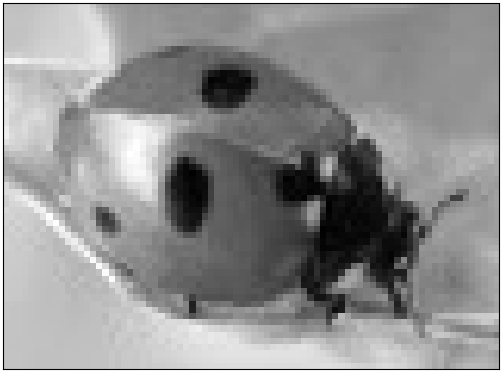
\includegraphics[scale=.25]{imagens/joaninha.png}
%\caption{\tiny{\url{https://commons.wikimedia.org/wiki/File:5-stip_LHB_09.jpg}}}
\end{figure}
\end{center}

\column{.5\textwidth}
\begin{center}
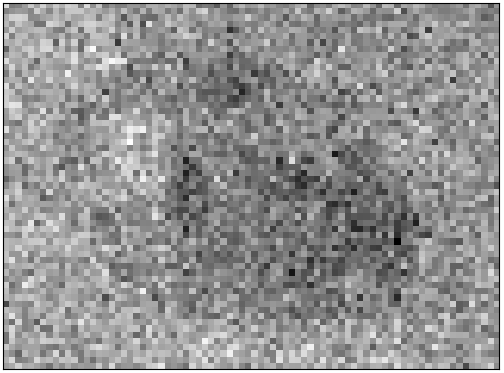
\includegraphics[scale=.25]{imagens/joaninhaMMQ_20porcento.png}
\end{center}
\end{columns}
\center{\tiny{Adaptado de \url{https://commons.wikimedia.org/wiki/File:5-stip_LHB_09.jpg}}}
\end{frame}

\begin{frame}
\frametitle{Compressive Sensing}
Imagens geralmente são esparsas no espectro da frequência.

\begin{columns}[t]
\column{.5\textwidth}
\begin{center}
\begin{figure}
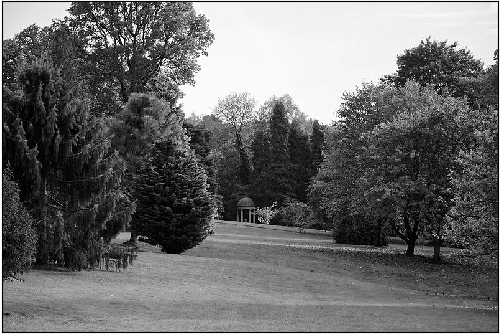
\includegraphics[scale=.4]{imagens/Beale_Arboretum_gray.png}
%\caption{\tiny{\url{https://commons.wikimedia.org/wiki/File:Along_The_Main_Ride_-_Beale_Arboretum}}}
\end{figure}
Imagem original
\end{center}

\column{.5\textwidth}
\begin{center}
\begin{figure}
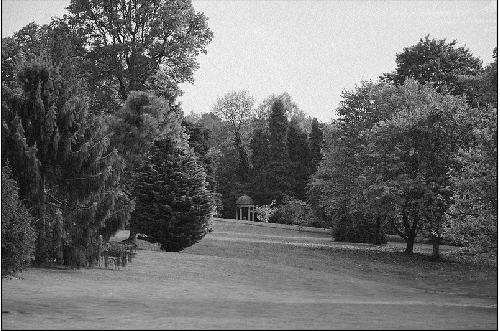
\includegraphics[scale=.4]{imagens/Beale_Arboretum_60porc_freq_maiores.png}
%\caption{Compressão de $40%$}
\end{figure}
Compressão de $40\%$
\end{center}
\end{columns}
\center{\tiny{Adaptado de \url{https://commons.wikimedia.org/wiki/File:Along_The_Main_Ride_-_Beale_Arboretum}}}
\end{frame}

\begin{frame}
\frametitle{Compressive Sensing}
Queremos encontrar $x$ mais esparso com $Ax = y$, ou seja,
\begin{equation}
\min_{x \in \mathbb{R}^n} \Vert x \Vert_0 \textit{ sujeito a } Ax = y
\tag{$P_0$}
\label{eqn:P0}
\end{equation}

onde $\Vert x \Vert_0$ é a quantidade de elementos não nulos de $x$. \\

Mas $\eqref{eqn:P0}$ é não pode ser resolvido em tempo polinomial.
\end{frame}

\begin{frame}
\frametitle{Compressive Sensing}
\begin{center}
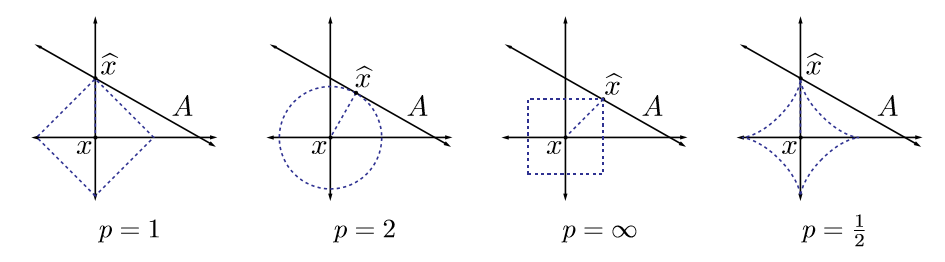
\includegraphics[scale=.4]{imagens/normas.png}

\tiny{Davenport, Mark A., et al. "Introduction to compressed sensing." Preprint 93.1 (2011): 2.}
\end{center}
\begin{equation}
\min_{x \in \mathbb{R}^n} \Vert x \Vert_p \textit{ sujeito a } Ax = y
\tag{$P_p$}
\label{eqn:Pp}
\end{equation}
\end{frame}

\begin{frame}
\frametitle{Compressive Sensing}
Compressive Sensing estuda as condições que $A$ deve satisfazer para garantir a equivalência entre

\begin{equation}
\min_{x \in \mathbb{R}^n} \Vert x \Vert_0 \textit{ sujeito a } Ax = y
\tag{$P_0$}
%\label{eqn:P0}
\end{equation}

e

\begin{equation}
\min_{x \in \mathbb{R}^n} \Vert x \Vert_1 \textit{ sujeito a } Ax = y
\tag{$P_1$}
\label{eqn:P1}
\end{equation}
\end{frame}

\begin{frame}
\frametitle{Compressive Sensing}
Uma dessas condições leva em conta a coerência de $A$, definida como

$$\mu(A) = \max_{i \neq j} \vert \langle a_i, a_j \rangle \vert$$

\begin{center}
\begin{columns}[t]
\column{.5\textwidth}
\vspace{.5cm}
\begin{center}
\begin{tikzpicture}[thick]
\begin{scope}[-stealth]
%    \draw [blue   ] (0,7.5) -- (1,7.5) node [right] {stealth};;
%    \draw [red,   ] (0,7.0) -- (1,7.0) node [right] {stealth};
%    \draw [brown,-] (0,6.5) -- (1,6.5);
	\draw [gray ]  (0,-1) -- (0,.5) node [right] {$a_1$};
	\draw [gray ]  (0,-1) -- (1,-.7) node [right] {$a_2$};
	\draw [gray ]  (0,-1) -- (1.5,-1) node [right] {$a_3$};
	\draw [gray ]  (0,-1) -- (-.6,.1) node [right] {$a_4$};
	\draw [black ] (0,-1) -- (.2,0) node [right] {$y$};
\end{scope}
\end{tikzpicture}
\end{center}
\column{.5\textwidth}
\begin{center}
Note que
%$$y = Ax = \sum_{i = 1}^n a_i \langle a_i, x \rangle$$
$$y = Ax = \sum_{i = 1}^n a_i x_i$$
\end{center}
\end{columns}
\end{center}

\end{frame}

\begin{frame}
\frametitle{Compressive Sensing}
$A$, com $a_{ij} \sim \mathcal{N}(0,1)$ independentes, satisfaz essas condições com alta probabilidade.
\end{frame}

\begin{frame}
\frametitle{Compressive Sensing}
\framesubtitle{Algoritmo de homotopia}
Resolve $\eqref{eqn:P1}$ encontrando uma sequência $(x_n)$ de soluções para

$$J_n(x) = \Vert Ax - y \Vert_2^2 + \lambda_n \Vert x \Vert_1$$

com $(\lambda_n)$ decrescente.
\end{frame}

\begin{frame}
\frametitle{Compressive Sensing}
\framesubtitle{Algoritmo de homotopia}
\begin{center}
Imagens recuperadas com taxa de compressão de $20\%$\\
\end{center}

\begin{columns}[t]
\column{.33\textwidth}
\centering
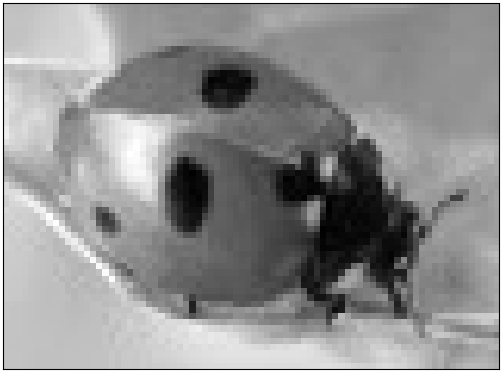
\includegraphics[scale=.25]{imagens/joaninha.png}\\
Imagem original

\column{.33\textwidth}
\centering
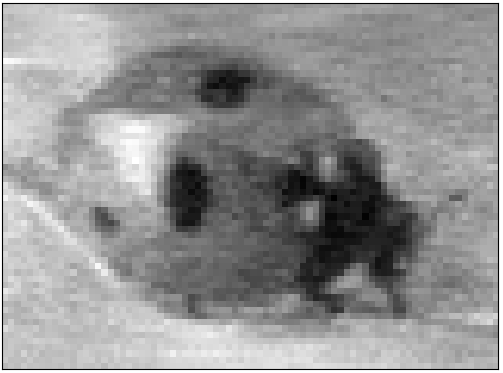
\includegraphics[scale=.25]{imagens/joaninhaHomotopy_20porcento.png}\\
Homotopia

\column{.33\textwidth}
\centering
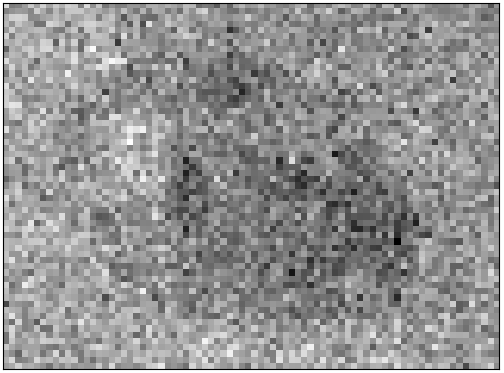
\includegraphics[scale=.25]{imagens/joaninhaMMQ_20porcento.png}\\
Mínimos quadrados
\end{columns}
\center{\tiny{Adaptado de \url{https://commons.wikimedia.org/wiki/File:5-stip_LHB_09.jpg}}}
\end{frame}

\begin{frame}
\frametitle{Compressive Sensing}
\framesubtitle{O modelo cross-and-bouquet}

Dada uma matriz

$$ A = \left[ \raisebox{-4pt}{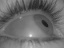
\includegraphics[scale=.3]{imagens/olhos/(0,0).jpg}} \vert \raisebox{-4pt}{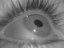
\includegraphics[scale=.3]{imagens/olhos/(2,4).jpg}} \vert \raisebox{-4pt}{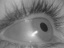
\includegraphics[scale=.3]{imagens/olhos/(4,1).jpg}} \vert \cdots \vert \raisebox{-4pt}{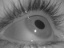
\includegraphics[scale=.3]{imagens/olhos/(6,4).jpg}}  \right]$$

e um vetor

$$y = \left[ \raisebox{-4pt}{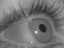
\includegraphics[scale=.3]{imagens/olhos/(5,2).jpg}} \right]$$

qual é a coluna de $A$ (amostra) mais parecida com $y$?
\end{frame}

\begin{frame}
\frametitle{Compressive Sensing}
\framesubtitle{O modelo cross-and-bouquet}

Vamos formular essa pergunta como um problema de Compressive Sensing.

$$y = Ax + e = \left[ \begin{tabular}{c | c} A & I \end{tabular} \right] \left[ \begin{tabular}{c} x \\ e \end{tabular}\right] = Bc$$

$$\min_{c \in \mathbb{R}^n} \Vert c \Vert_1 \textit{ sujeito a } Bc = y$$
\end{frame}

\begin{frame}
\frametitle{Compressive Sensing}
\framesubtitle{O modelo cross-and-bouquet}
\centering
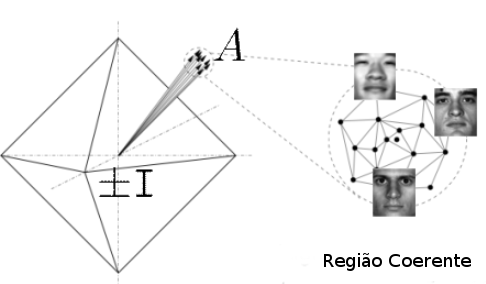
\includegraphics[scale=.4]{imagens/cross-and-bouquet.png}

\tiny{Yang, Allen Y., et al. A Review of Fast L (1)-Minimization Algorithms for Robust Face Recognition. CALIFORNIA UNIV BERKELEY DEPT OF ELECTRICAL ENGINEERING AND COMPUTER SCIENCE, 2010.}
\end{frame}

\begin{frame}
\frametitle{Compressive Sensing}
\framesubtitle{O modelo cross-and-bouquet}
\centering
Identificaremos a amostra $a_i$ mais próxima de $y$ satisfazendo

$$i = \arg \max_{1 \leq i \leq n} \vert x_i \vert$$
\end{frame}

\begin{frame}
\frametitle{Desenvolvimento de um rastreador de olhar}

Usamos uma câmera da Pupil Labs

\vspace{1cm}
\centering
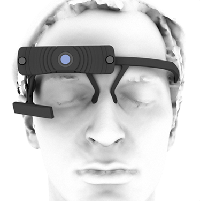
\includegraphics[scale=.6]{imagens/pupil.png}

\tiny{\url{https://pupil-labs.com/blog/2016-07/new-headset-color/}}
\end{frame}

\begin{frame}
\frametitle{Desenvolvimento de um rastreador de olhar}
\framesubtitle{Coleta}

Coletamos imagens do olho direito de $6$ participantes.
\centering
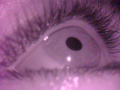
\includegraphics[scale=1]{imagens/26.jpg}
\end{frame}

\begin{frame}
\frametitle{Desenvolvimento de um rastreador de olhar}
\framesubtitle{Coleta}

\centering

\includegraphics[scale=.6]{imagens/alvo.png}
\end{frame}

\begin{frame}
\frametitle{Desenvolvimento de um rastreador de olhar}
\framesubtitle{Rastreamento}

Escolhemos a primeira imagem registrada para cada alvo, reduzimos a imagem e calculamos a matriz $A$.

$$ A = \left[ \raisebox{-4pt}{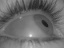
\includegraphics[scale=.3]{imagens/olhos/(0,0).jpg}} \vert \raisebox{-4pt}{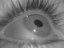
\includegraphics[scale=.3]{imagens/olhos/(2,4).jpg}} \vert \raisebox{-4pt}{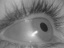
\includegraphics[scale=.3]{imagens/olhos/(4,1).jpg}} \vert \cdots \vert \raisebox{-4pt}{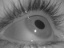
\includegraphics[scale=.3]{imagens/olhos/(6,4).jpg}}  \right]$$
\end{frame}

\begin{frame}
\frametitle{Desenvolvimento de um rastreador de olhar}
\framesubtitle{Rastreamento}

Escolhemos $5$ imagens por alvo e estimamos a posiçao do olhar para cada imagem.
\end{frame}

\begin{frame}
\frametitle{Desenvolvimento de um rastreador de olhar}
\framesubtitle{Rastreamento}
$$ A = \left[ \raisebox{-4pt}{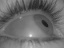
\includegraphics[scale=.3]{imagens/olhos/(0,0).jpg}} \vert \raisebox{-4pt}{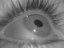
\includegraphics[scale=.3]{imagens/olhos/(2,4).jpg}} \vert \raisebox{-4pt}{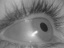
\includegraphics[scale=.3]{imagens/olhos/(4,1).jpg}} \vert \cdots \vert \raisebox{-4pt}{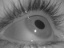
\includegraphics[scale=.3]{imagens/olhos/(6,4).jpg}}  \right]$$

$$y = \left[ \raisebox{-4pt}{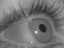
\includegraphics[scale=.3]{imagens/olhos/(5,2).jpg}} \right]$$

$$y = Ax + e$$

Calculamos o olhar como a média ponderada das posições das três amostras mais próximas de $y$.
\end{frame}

\begin{frame}
\frametitle{Compressive Sensing}
\framesubtitle{Rastreamento}

Poderíamos estimar a amostra mais parecida com $y$ como a coluna $a_i$ que maximiza, em módulo, a correlação entre $y$ e $a_i$.\\


Fizemos um teste para identificar a posição do olho e taxa de acerto foi de $14,286\%$.
\end{frame}

\begin{frame}
\frametitle{Compressive Sensing}
\framesubtitle{Rastreamento}

\centering
Taxa de acertos para identificar imagens
\footnotesize{
\begin{table}
\begin{tabular}{| c | c | c | c |}
\hline
proporções da imagem & correlação & \textit{cross-and-bouquet} \\ \hline
$640 \times 480$ & $14,29\%$	 & ---\\ \hline
$320 \times 240$ & $12,25\%$	 & ---\\ \hline
$160 \times 120$ & $10,20\%$	 & ---\\ \hline
$80 \times 60$   & $8,16\%$		 & $90,61\%$ \\ \hline
$40 \times 30$	 & $6,12\%$		 & $91,02\%$ \\ \hline
$20 \times 15$	 & $2,04\%$		 & $86,94\%$ \\ \hline
\end{tabular}
\end{table}
}
\end{frame}

\begin{frame}
\frametitle{Desenvolvimento de um rastreador de olhar}
\framesubtitle{Resultados}

\begin{center}
Desempenho do rastreador para diferentes resoluções de imagem
\end{center}
%\footnotesize{
\scriptsize{
\begin{table}
\centering
\begin{tabular}{ c  c  c  c }
\hline
Dimensões das imagens & $15 \times 20$ & $30 \times 40$ & $60 \times 80$ \\ \hline
Erro				  & $1,471 \pm 2,398$ & $1,113 \pm 2,291$ & $1,053 \pm 2,279$ \\ \hline
Imagem & \vspace{2pt} \raisebox{-16pt}{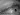
\includegraphics[width=1cm]{imagens/olho_20_15.jpg}} & \raisebox{-16pt}{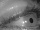
\includegraphics[width=1cm]{imagens/olho_40_30.jpg}} & \raisebox{-16pt}{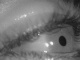
\includegraphics[width=1cm]{imagens/olho_80_60.jpg}} \\ \hline
Tempo necessário & $13,46$s & $55,42$s & $22,98$ min \\ \hline
\end{tabular}
\end{table}
}
\centering
\footnotesize{O rastreador apresenta desempenho semelhante ao Eyex ( $1,42 \pm 1,7$)}
\end{frame}

\begin{frame}
\frametitle{Desenvolvimento de um rastreador de olhar}
\framesubtitle{Resultados}

%\begin{center}
%Acurácia por posição na tela
%\end{center}

\begin{columns}[t]
\column{.5\textwidth}
\centering
\tiny{usando imagens $15 \times 20$}
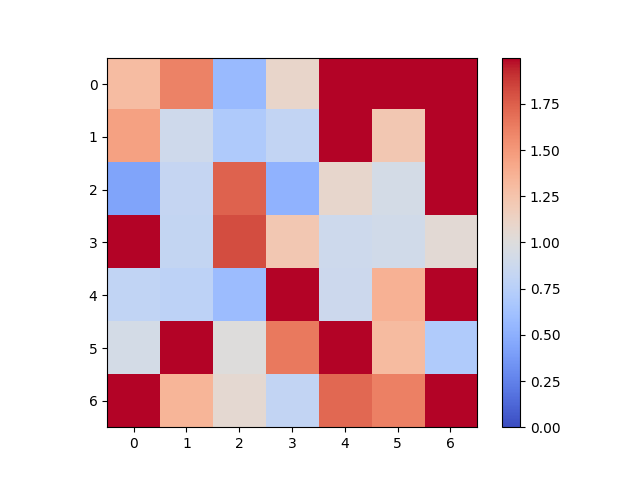
\includegraphics[scale=.25]{imagens/erros5pyrDown.png}

%\column{.5\textwidth}
%\centering
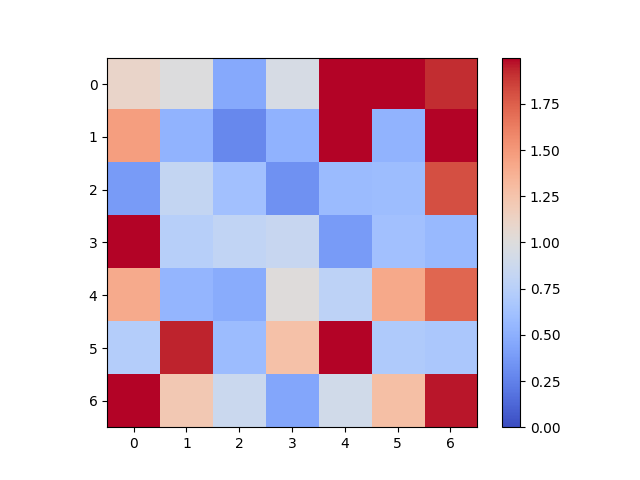
\includegraphics[scale=.25]{imagens/erros4pyrDown.png}

\tiny{usando imagens $30 \times 40$}

\column{.5\textwidth}
\centering
\tiny{usando imagens $60 \times 80$}
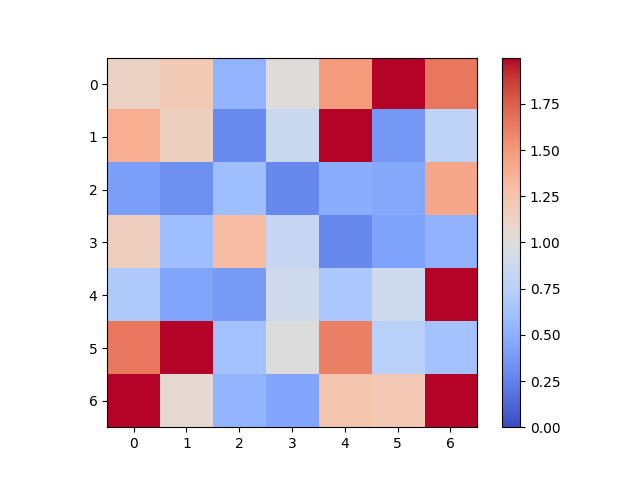
\includegraphics[scale=.25]{imagens/erros3pyrDown.png}
\end{columns}
\end{frame}

\begin{frame}
\frametitle{Desenvolvimento de um rastreador de olhar}
\framesubtitle{Resultados}

%\begin{center}
%Erros por participante
%\end{center}
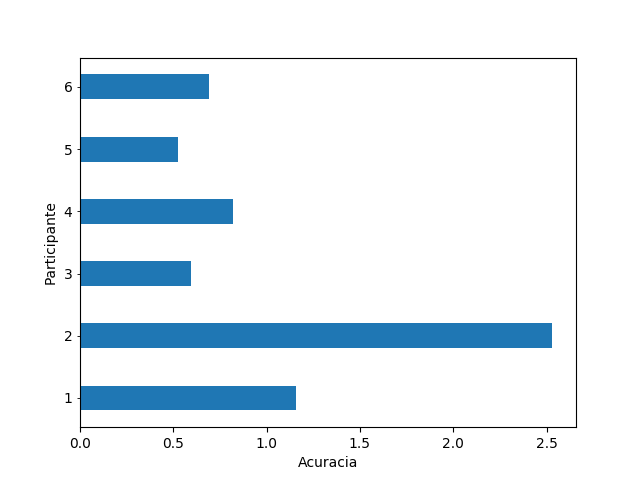
\includegraphics[scale=.65]{imagens/errosParticipantes_pyrDown3.png}
\end{frame}

\begin{frame}
\frametitle{Conclusão}
\begin{itemize}
\item Neste trabalho estudamos conceitos de rastreamento de olhar e Compressed Sensing
\item Elaboramos um experimento para testar o desempenho do rastreador
\item Apesar das limitações, o rastreador apresenta desempenho semelhante a um rastreador comercial
\end{itemize}
\end{frame}
\end{document}